\begin{figure}[h]
	\hspace{-0.25\textwidth}
	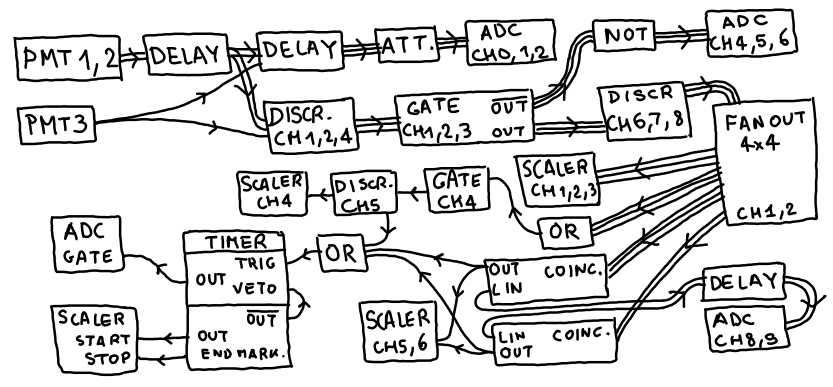
\includegraphics[width=0.9\textwidth]{immagini/circuitone}~
	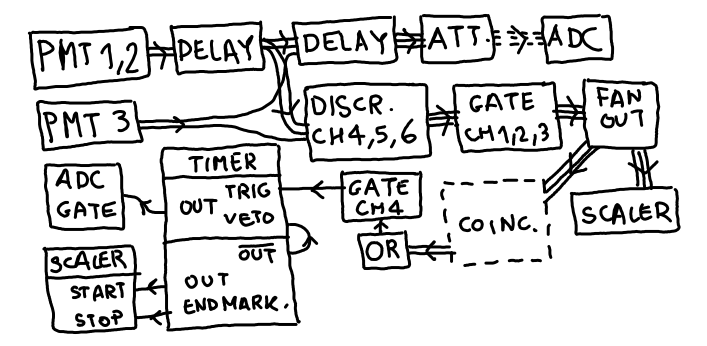
\includegraphics[width=0.6\textwidth]{immagini/circuitob}
	\caption{Circuito dell'apparato A (sinistra) e dell'apparato B (destra).}
	\label{circuitone}
\end{figure}

\subsection{Circuito A}

\subsubsection{Descrizione del circuito}

Il primo circuito assemblato è rappresentato in \autoref{circuitone}.

Le uscite dei PMT sono inviate ai discriminatori, le cui uscite attraversano un modulo di antiretrigger (tempo morto di \SI{1}{\micro s}) e vengono usate per costruire funzioni logiche. I segnali dei PMT vengono anche inviati all'ADC attraverso un attenuatore per regolare il fondoscala.

Per quanto riguarda la parte logica, costruiamo e mettiamo in tempo tre tipi di trigger:
\begin{enumerate}
\item canale
\item coincidenza a 2
\item coincidenza a 3.
\end{enumerate}
Il trigger di canale è semplicemente il segnale discriminato del PMT corrispondente; quello di coincidenze è dato dall'uscita di lunga durata del modulo stesso. Mandiamo questi segnali all'ADC in modo che il trigger di canale arrivi in contemporanea con il segnale analogico del canale stesso. Se in quel momento c'è anche un trigger di coincidenza, sappiamo se l'evento ci è arrivato da una coincidenza anziché da un canale singolo. Abbiamo fatto tutto questo per acquisire tutti i canali contemporaneamente ed agevolare la lettura dei dati via software. Purtroppo il \emph{crosstalk}%
\footnote{Spiegheremo come ci siamo accorti di questo problema nella \autoref{ref}.} presente nell'ADC ha rovinato le misure fatte con questo circuito.

\marginpar{``Rovinato'' non mi piace tanto.}

Per dare precedenza agli eventi più rari abbiamo collegato questi trigger ad un modulo \emph{or} ritardando i trigger singoli rispetto a quelli di coincidenze a 2 e questi ultimi rispetto alle coincidenze a 3. L'uscita dell'\emph{or} era poi inviata ad un \emph{timer} che generava il gate dell'ADC. L'altro canale di questo \emph{timer} veniva usato per avviare o fermare le acquisizioni.

\subsubsection{Problemi riscontrati}

Purtroppo il circuito presentava dei problemi.

Il più evidente fin da subito è stato il \emph{bit stuck}: il terzo bit meno significativo dei dati in formato binario è sempre 1.
Gli istogrammi presentano delle lacune di \SI{4}{digit} ogni \SI{4}{digit}. Risolviamo questo problema usando canali del tipo $[0,8n) , n \in \mathcal{N}$ nei vari istogrammi.
Poi abbiamo escluso l'\emph{or} dal circuito perché i segnali che ci arrivavano dalle coincidenze mostravano avere un'energia minore. Abbiamo risolto il problema togliendo l'\emph{or} dal circuito.
\marginpar{Spiegare perché: che la temporizzazione è diversa,
che il modulo gate ha jitter eccessivo per tempi $>\SI{1}{ms}$.}

Il problema più interessante è dato dal fatto che, confrontando gli spettri del \na{}, abbiamo visto che i fotoni emessi dalla sorgente con attività maggiore avevano energia maggiore.
Il grafico in \autoref{distanze} mostra l'energia dei fotopicchi del sodio in funzione del rate misurato ponendo la sorgente ad attività elevata a varie distanze dal rivelatore.
I dati della misura si trovano \autoref{tabella forte}.

\begin{figure}[h]
\centering
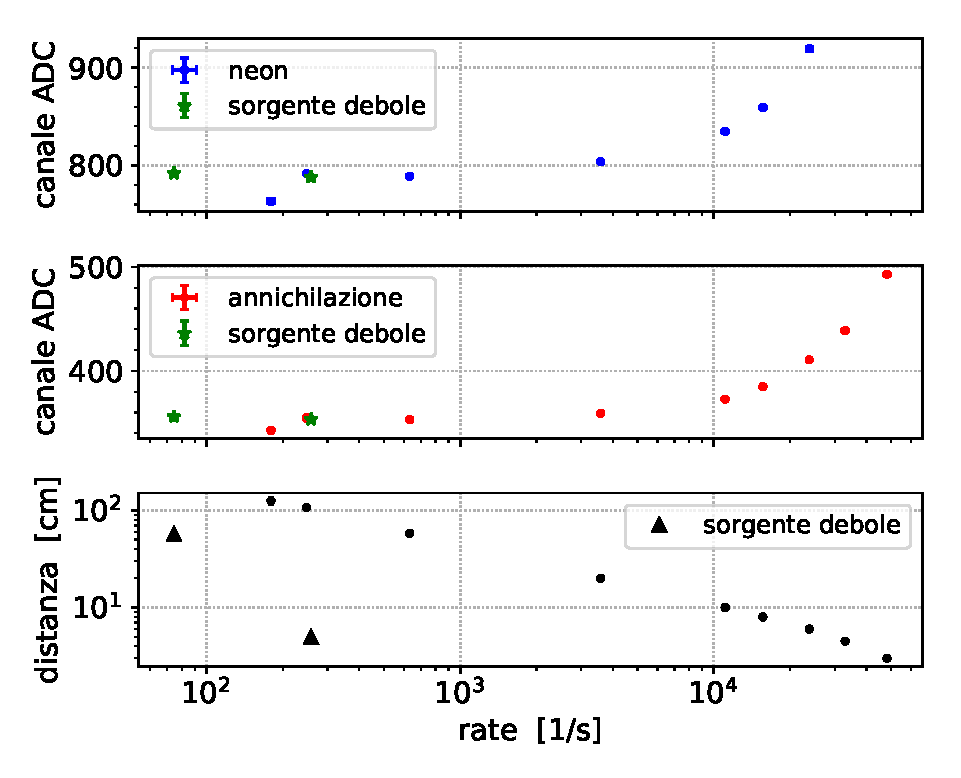
\includegraphics[width=28 em]{immagini/naforte}
\caption{Posizione dei fotopicchi del sodio in funzione del rate di eventi ponendo la sorgente a diverse distanze dal rivelatore. In alcune delle acquisizioni non era visibile il picco del neon oppure era talmente deformato da rendere privo di senso il fit gaussiano. La linea tratteggiata mostra la posizione dello stesso picco usando la sorgente di attività minore.}
\label{distanze}
\end{figure}

\begin{table}[h]
\centering
\begin{tabular}{c|c|c}
rate [1/s] & beta [digit] & neon [digit] \\
\hline
 179.5$\,\pm\,$0.2 & 342.86$\,\pm\,$0.52 & 763.4$\,\pm\,$2.4 \\
 247.7$\,\pm\,$0.2 & 354.76$\,\pm\,$0.45 & 791.7$\,\pm\,$1.3 \\
 632.8$\,\pm\,$0.2 & 353.26$\,\pm\,$0.35 & 788.8$\,\pm\,$1.4 \\
3583.7$\,\pm\,$0.7 & 359.26$\,\pm\,$0.39 & 803.7$\,\pm\,$1.1 \\
  11086$\,\pm\,$14 & 372.79$\,\pm\,$0.24 & 834.8$\,\pm\,$1.0 \\
  15613$\,\pm\,$15 & 384.92$\,\pm\,$0.27 & 859.16$\,\pm\,$0.97 \\
  23784$\,\pm\,$24 & 410.76$\,\pm\,$0.45 & 919.4$\,\pm\,$2.5 \\
  32948$\,\pm\,$27 & 438.8$\,\pm\,$1.2 &         \\
  48190$\,\pm\,$24 & 492.90$\,\pm\,$0.76 &        
\end{tabular}

\caption{Tabella dei dati in \autoref{distanze}. ``Beta'' indica la media del picco di annichilazione ``neon'' quella del relativo fotopicco.}
\label{tabella forte}
\end{table}

Pensiamo che tale effetto sia dovuto ad un pile-up nella digitalizzazione in quanto l'ADC ha un tempo di conversione di \SI{60}{\micro s}.
\marginpar{Dalle misure fatte l'ultimo giorno sappiamo che
il problema non può essere solo il pile-up della digitalizzazione.
Inoltre avevamo anche escluso che il problema fosse solo il pile-up dei segnali.}
Dal grafico si evince che anche con un rate di eventi minore di \SI{10}{ms^{-1}} il problema persiste perché la distribuzione temporale tra un evento e il successivo non è uniforme, ma esponenziale. Quindi tra due eventi consecutivi intercorre spesso un piccolo intervallo di tempo.
Abbiamo quindi deciso di utilizzare la sorgente ad attività minore per misurare la massa dell'elettrone e quella ad attività maggiore per le misure in cui non ci interessa l'energia degli eventi o cerchiamo eventi rari.